%--------------------------------------------------------------------
%--------------------------------------------------------------------
% Formato para los talleres del curso de Herramientas Computacionales
% Universidad de los Andes
% 2015-10
%--------------------------------------------------------------------
%--------------------------------------------------------------------

\documentclass[11pt,letterpaper]{exam}
\usepackage[utf8]{inputenc}
\usepackage[spanish]{babel}
\usepackage{graphicx}
\usepackage{mdframed}
\usepackage{tabularx}
\usepackage[absolute]{textpos} % Para poner una imagen completa en la portada
\usepackage{multirow}
\mdfdefinestyle{mystyle}{leftmargin=1cm,rightmargin=1cm,linecolor=red}
\usepackage{float}
\usepackage{hyperref}
\decimalpoint
%\usepackage{pst-barcode}
%\usepackage{auto-pst-pdf}

\newcommand{\base}[1]{\underline{\hspace{#1}}}
\boxedpoints
\pointname{ pt}
%\extrawidth{0.75in}
%\extrafootheight{-0.5in}
\extraheadheight{-0.15in}
%\pagestyle{head}

%\noprintanswers
%\printanswers
\renewcommand{\solutiontitle}{}
\SolutionEmphasis{\color{blue}}

\usepackage{upquote,textcomp}
\newcommand\upquote[1]{\textquotesingle#1\textquotesingle} % To fix straight quotes in verbatim

\begin{document}
\begin{center}
{\Large Herramientas Computacionales} \\
Taller 3 - \LaTeX (2)\\
Fecha de publicación: {\small \it febrero 18 de 2015}\\
\end{center}

\begin{textblock*}{40mm}(10mm,20mm)
  
\includegraphics[width=3cm]{logoUniandes.png}
\end{textblock*}

\begin{textblock*}{40mm}(161mm,20mm)
  
\includegraphics[width=3cm]{logoUniandes.png}
\end{textblock*}

\vspace{0.5cm}

La entrega de esta tarea debe contener los siguientes archivos: \verb'eldicto.sh', \verb'imagenes.tex' y \verb'referencias.tex'. Nombrar el archivo comprimido con el formato \verb'NombreApellido_HW3.tar.gz'\\

\begin{questions}

\question[35] (Listas) El archivo \verb|laletraa.txt| tiene las palabras que comienzan con la letra a. Cada línea del archivo tiene el nombre de la palabra y su definición, ambas separadas por dos punto y coma seguidos ;;. Haga un script \verb+eldicto.sh+ que tome el archivo con las definiciones, construya un archivo de \LaTeX \,\,y lo compile de tal forma que al final el resultado sea similar al que se muestra en el archivo adjunto \verb+eldicto.pdf+. IMPORTANTE: utilice \verb+xelatex+ para compilar y añada las líneas 

\verb+\usepackage{fontspec,xltxtra,xunicode}+ 

y

\verb+\setmainfont{Times New Roman}+

al inicio del documento de \LaTeX. Debe usar el ambiente \verb|description|. 

Para resolver este ejercicio puede hacer uso del comando \verb|sed|. Tenga en cuenta lo siguiente:

\begin{itemize}
\item \verb"sed 's/símbolo-a-quitar/símbolo-a-insertar/g'"\\
Toma el archivo de entrada y lo imprime con todas las ocurrencias del símbolo-a-quitar reemplazadas con el símbolo-a-insertar, los caracteres \verb+\+ y \verb+&+ son especiales y deben usarse como se explica más adelante.
\item \verb"sed 's/$/final/g'" \\
Toma el archivo de entrada y pone al final de cada línea el texto ``final''.
\item \verb"sed 's/^/inicio/g'" \\
Toma el archivo de entrada y pone al inicio de cada línea el texto ``inicio''.
\item Si quiere usar el caracter \verb+\+ en \verb+sed+ como parte de un texto tiene que ponerlo de la forma \verb+\\+, por ejemplo, si al final de cada línea quisiera poner \verb+\final+, debería invocar \verb+sed+ de la siguiente forma \verb+sed 's/$/\\final/g'+
\end{itemize}

\newpage

\question[30] (Imágenes) Hacer un archivo \verb"imagenes.tex" que reproduzca lo que se muestra abajo, en la parte donde se hace referencia a la figura (fig.\ 1) no vale escribir literalmente ``fig.\ 1'', tiene que usar el comando \verb+\ref+. 

\DeclareGraphicsExtensions{.pdf,.png,.jpg}

\begin{mdframed}[style=mystyle]
\vspace{0.5cm}
En la fig.\ \ref{fig:Isaac} se muestra un retrato de \textit{Sir Isaac Newton}.

\begin{figure}[H]
\centering
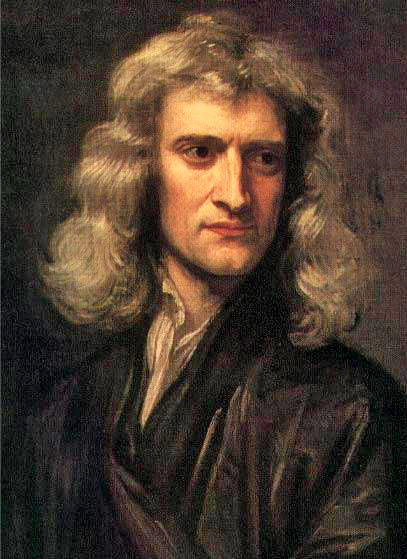
\includegraphics[scale=0.3]{isaac}
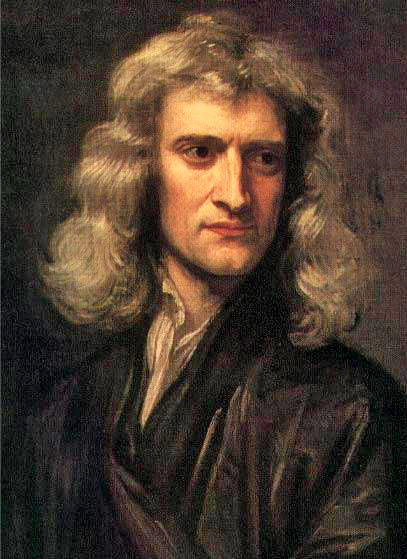
\includegraphics[scale=0.2]{isaac}
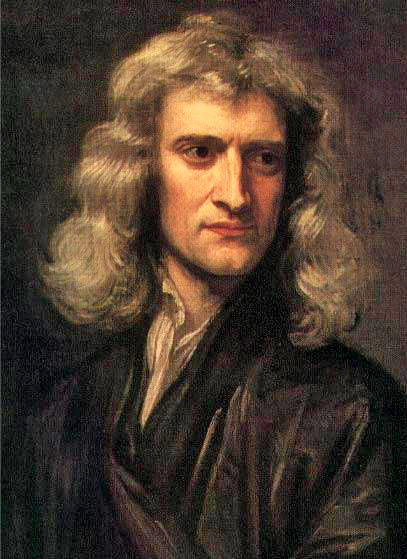
\includegraphics[scale=0.2, angle=100]{isaac}
\caption{Retrato de \textit{Sir Isaac Newton}.}
\label{fig:Isaac}
\end{figure}
\end{mdframed}

\question[35] {(Bibliograf\'ia)} En el archivo \verb"referencias.bib" se encuentra la bibliografía del documento \verb|articulo.pdf|. Cree el archivo \verb+referencias.tex+ donde se reproduzcan los primeros dos p\'arrafos de la introducci\'on del documento \verb|articulo.pdf| con las debidas referencias (excepto la referencia [10]) luego de invocar \verb+pdflatex - bibtex - pdflatex - pdflatex+. En el archivo que se genera, los n\'umeros de las referencias no van a coincidir con los de \verb|articulo.pdf| debido a que no se usan todas las entradas del archivo \verb|referencias.bib|. Aseg\'urese de que en el archivo de \LaTeX \hspace{2pt}utilice los comandos \verb+\bibliography+,\\ \verb+\bibliographystyle+ y \verb+\cite+.

\end{questions}

\end{document}